\chapter{Elementos finitos para biomecánica: problemas lineales}
\label{cap2}

\section{Objetivos de la práctica}
\label{sec:objetivos}

En esta práctica se desarrolla la simulación mediante elementos finitos del comportamiento de materiales biológicos que se rigen por un modelo elástico lineal de comportamiento. La herramienta empleada es el programa \emph{FEBio} \cite{FEBiO}. Se supone que al inicio de la práctica se tendrán ciertas destrezas de manejo de la suite \emph{FEBio Studio}, las cuales se habrán adquirido de el seguimiento de la práctica 8.2. 

El problema a llevar a cabo se realizará con la geometría de un fémur real, suponiendo dos tipos de materiales elásticos de distinta rigidez y diferentes estados de carga. Este caso supone una aplicación real con este tipo de materiales en biomecánica. 

Recordar que la suite se subdivide en 3 programas que a día de hoy se integran en una Suite denominada \emph{FEBiO Studio}.  Los 3 programas han sido desarrollados como código Open Source en la Universidad de Utah (USA). Se pueden instalar en una única instalación, desde un mismo archivo de instalación que se puede encontrar en la siguiente enlace para los diferentes sistemas operativos:

\url{http://stokes.mecanica.upm.es/MNUB/}
\begin{itemize}
\item \emph{Usuario:} mnub
\item \emph{Contraseña:} BioMecanica
\end{itemize}

Independientemente, se pueden descargar de la página web de la propia suite:

\url{https://febio.org/downloads/}\\

Las version con la que se va a trabajar en este curso, con la que se ha elaborado esta guía y se muestra estable, es la 1.0.3 para Windows, Linux y Mac. Es una versión que trabaja con FEBio 3.0.2.

\section{Base teórica: Sistema matricial y Elásticidad 3D}
\label{sec:teoria}
El problema que se plantea resolver en esta práctica tiene en cuenta que cada nodo tiene 3 grados de libertad, a diferencia del problema estudiado en la práctica anterior que era 1D. Por tanto, la variable a aproximar será un vector de desplazamientos nodales de $i$ grados de libertad:

\begin{equation}
u_{i}^{h}(x)=\sum_{a=1}^{N_{\text {nod }}} u_{i a} N_{a}(x)
\end{equation}

donde las funciones de forma se puedes escribir en forma matricial. Asimismo, las deformaciones pueden interpolarse con las derivadas de dichas funciones de forma de la siguiente manera:

\begin{equation}
\left(\varepsilon_{k l}\right)^{h}=\frac{1}{2} \sum_{b}\left(u_{k b} N_{b, l}+u_{l b} N_{b, k}\right)=\sum_{b} B_{l b} u_{k b},
\end{equation}

siendo $B_{l b}$ la matriz de gradiente de funciones de forma simétrica, que sirve para aproximar las deformaciones, pero también fuerzas internas y matriz de rigidez:

\begin{eqnarray}
F_{p a}^{\text {int }} &=& \int_{\mathcal{B}} B_{q a} \sigma_{p q} \, \mathrm{d} V \\
K_{p a r b}&=& \int_{\mathcal{B}} B_{q a} C_{p q r s} B_{s b} \,\mathrm{d} V
\end{eqnarray}

La tensión se definde por tanto con un tensor tridimensional, $\bm{\sigma}$, denominado tensor de tensiones de \textit{Cauchy}. $C_{p q r s}$ representa el tensor constitutivo de cuarto orden, tal que tensiones y deformaciones quedan relacionadas por él mismo de la forma:

\begin{equation}
\sigma=\mathbb{C}: \varepsilon,
\end{equation}

que para el caso de elasticidad 3D se define por:

\begin{equation}
\mathbb{C} \equiv C_{i j k l}=\lambda \delta_{i j} \delta_{k l}+2 \mu \delta_{i k} \delta_{j l}
\end{equation}

El último componente del sistema, las fuerzas externas, se puede definir en 3D por:

\begin{equation}
F_{p a}^{\text {ext }} = \int_{\partial_{t} \mathcal{B}} t_{p}^{*} N_{a} \mathrm{d} S+\int_{\mathcal{B}} q_{p} N_{a} \mathrm{d} V
\end{equation}

Por tanto, el sistema a resolver, similar al estudiado en una dimension, es:

\begin{equation}
[\mathbf{K}]\{\mathbf{u}\}=\{\mathbf{f}\}.
\end{equation}

Este sistema, para los ejemplos en 3D que se han referido en los objetivos del apartado~\ref{sec:objetivos}, se resolverán en la siguiente práctica con la suite \emph{FEBiO}, que se describe en el siguiente apartado.

\clearpage
\section{Simulación de un femur sometido a compresión}
\label{sec:femur}
Para los materiales estudiados en biomecánica, el caso de los tejidos oseos es el que mejor se aproxima al comportamiento elástico lineal. Una vez se ha trabajado con el programa en prácticas anteriores simplificados a una sola fibra elástica, podemos proceder al estudio de un problema con un hueso real.

Para ello, hemos de importar el archivo \texttt{FEMUR.feb} que está en Moodle. La forma de importarlo es seleccionando \emph{File/Open Model File}. Deberemos guardar el archivo como *.fsm para seguir trabajando con el mismo. Este tipo de archivo, FEBio Studio Model, es el que se guarda como global del proyecto.

\begin{figure}[!htp]
\centering
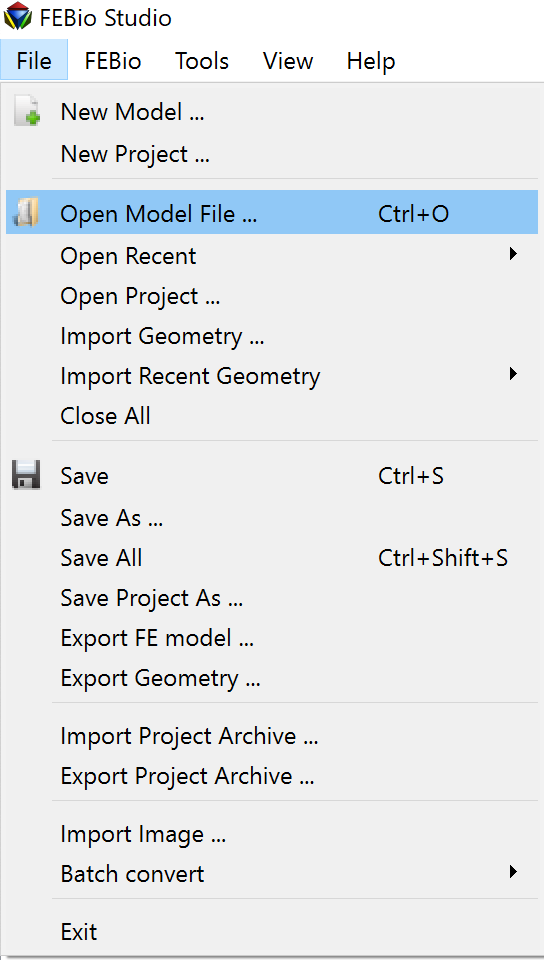
\includegraphics[width=0.25\textwidth]{figuras_2/import.png}
\caption{Abrir modelo de archivo *.feb}
\label{fig:femur0}
\end{figure}

Obtendremos algo similar al fémur de la figura~\ref{fig:femur1}. Como vemos, dicho modelo ya viene con la geometría y la malla de un fémur real, en milímetros. Además, en la sección \emph{Model}, vemos como existen dos materiales, denominados duro y blando. El primero se refiere a la parte de hueso compacto mientras que el segundo está asignado al hueso esponjoso.

\begin{figure}[!htp]
\centering
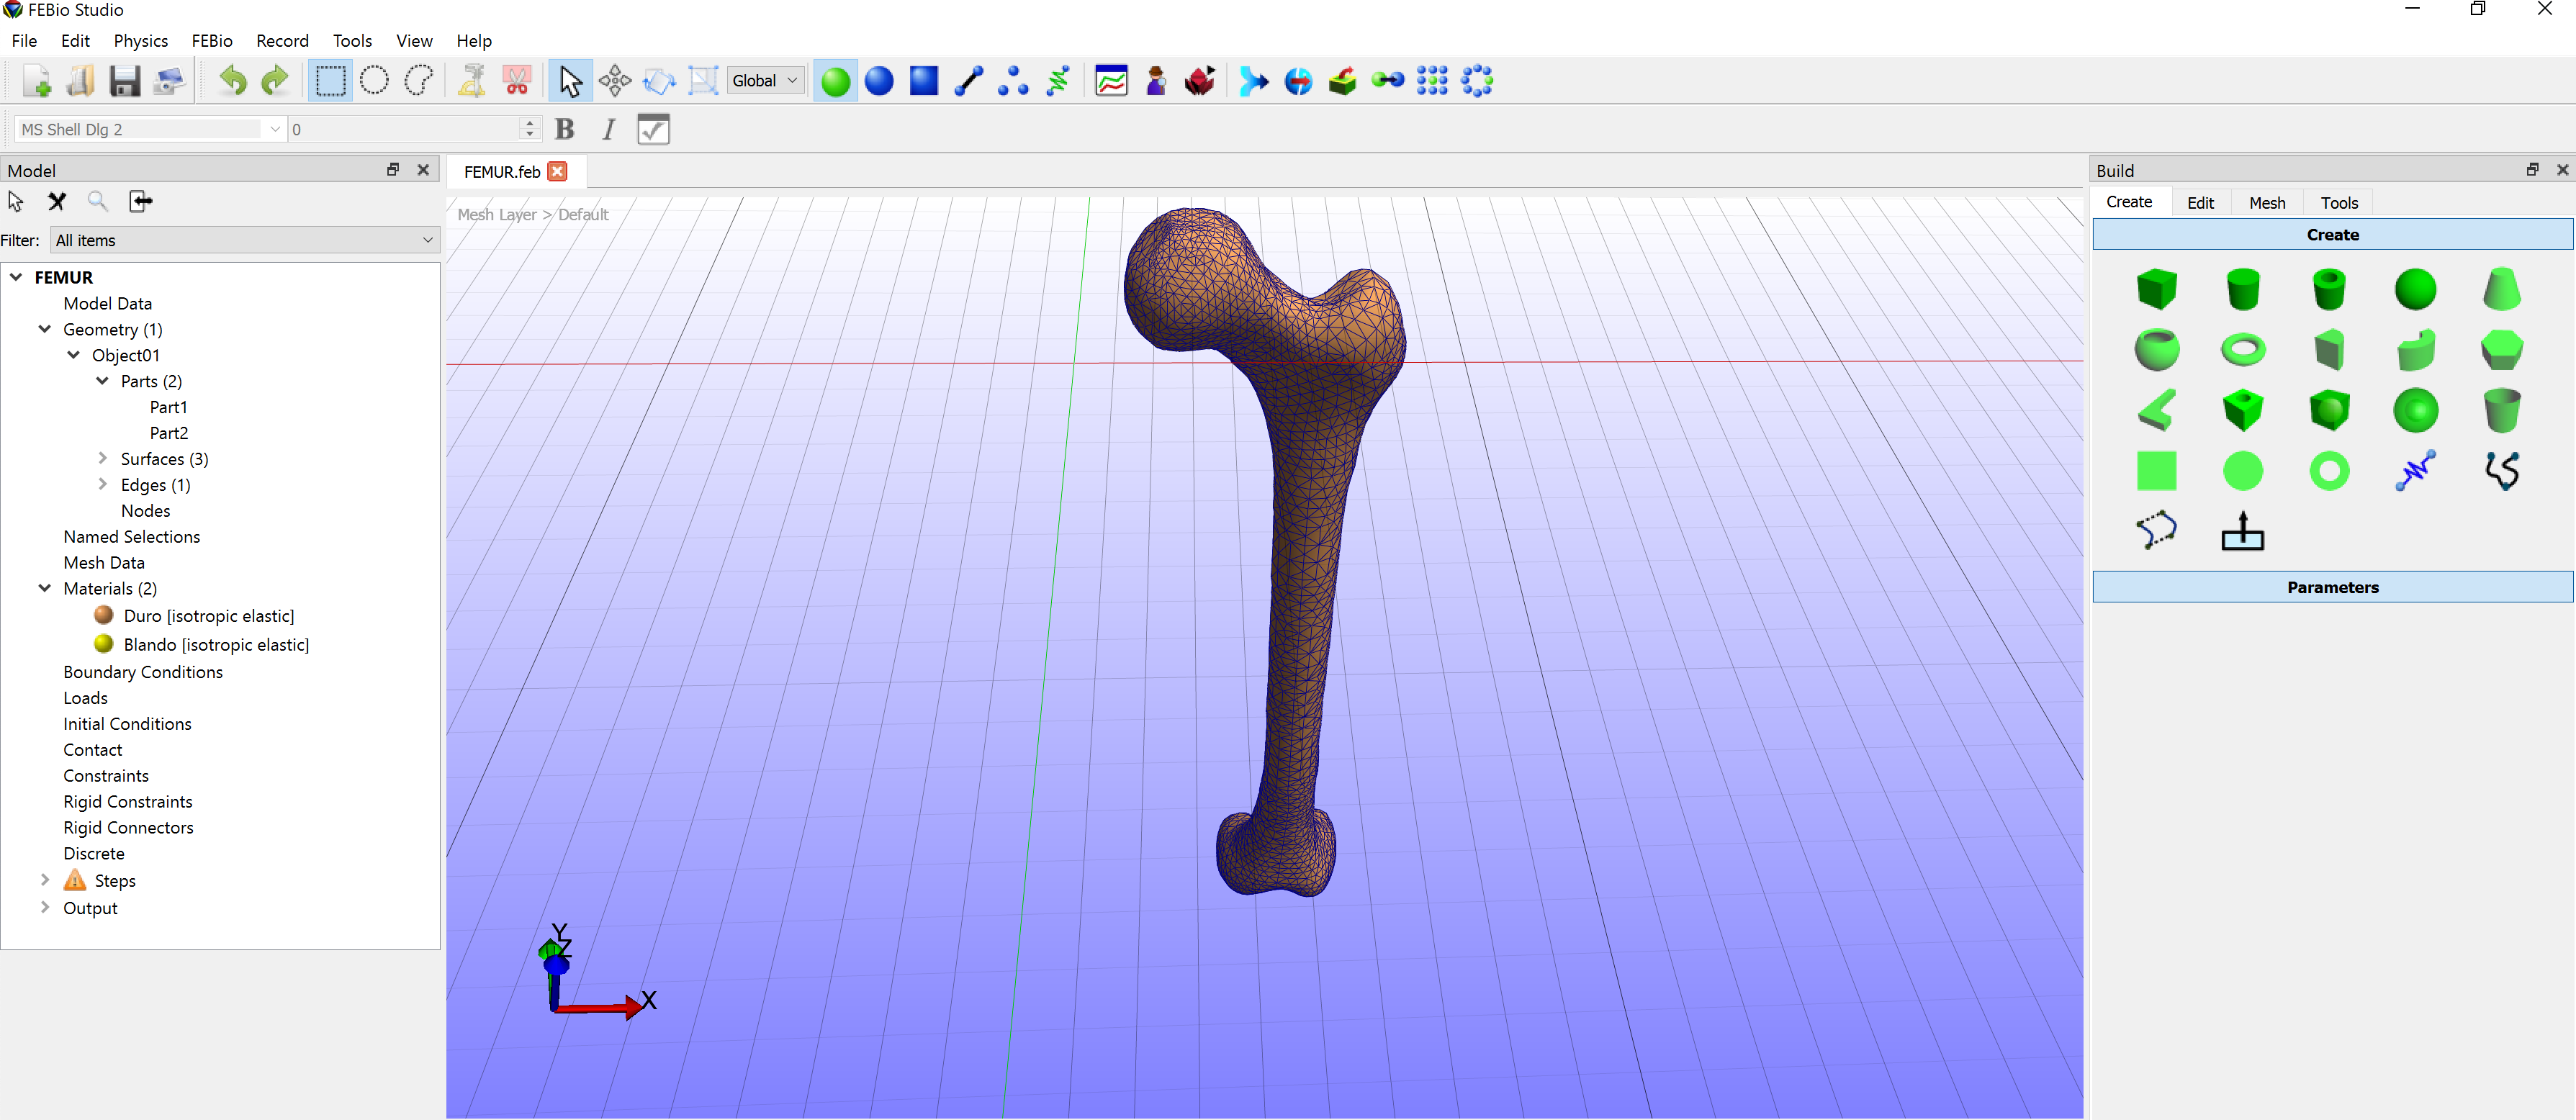
\includegraphics[width=0.85\textwidth]{figuras_2/femur1.png}
\caption{Modelo de fémur importado en \emph{FEBiO}}
\label{fig:femur1}
\end{figure}

Este modelo es el punto de partida para estudiar un caso real. Para ello debemos asignar las condiciones de contorno correspondientes al caso a resolver. Se ha planteado la idea de calcular las tensiones producidas por cargar el peso de un individuo de 100 kg desde la cadera. Para ello, fijaremos la articulación de la rodilla y cargaremos en la parte superior con una fuerza vertical de 1000 N. Para fijar la parte inferior, hemos de seleccionar los nodos correspondientes a estas zonas. En la figura~\ref{fig:femur2} vemos cómo hemos de, una vez seleccionado el objeto, activar la selección de nodos y la opción de seleccionar nodos adyacentes. Con un radio de acción de 20 y manteniendo pulsada la tecla mayúscula, seleccionamos en el punto central de cada una de las dos protusiones. Deberían quedar seleccionados una serie de nodos similar a los nodos señalados en rojo de la figura~\ref{fig:femur2}.

\begin{figure}[!htp]
\centering
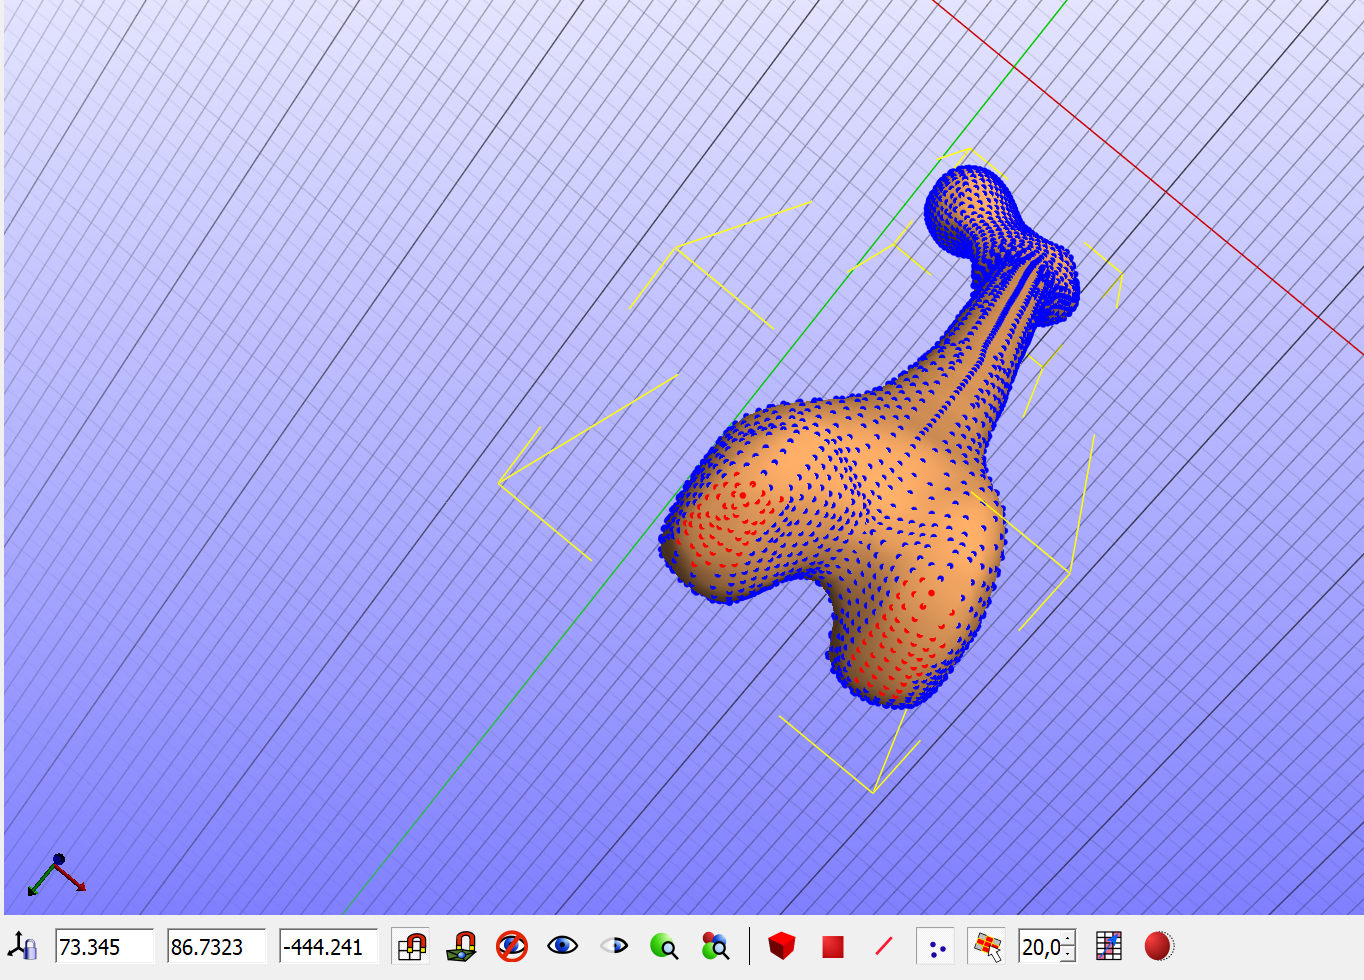
\includegraphics[width=0.75\textwidth]{figuras_2/femur2.png}
\caption{Selección de nodos a fijar.}
\label{fig:femur2}
\end{figure}
 
 Una vez seleccionados estos nodos se añadirá la condición de contorno en \textit{Physics/Add Boundary Condition} y procederemos a fijar los desplazamientos en las tres direcciones del espacio (\textit{Fixed Displacements}). 
 
 \begin{figure}[!htp]
\centering
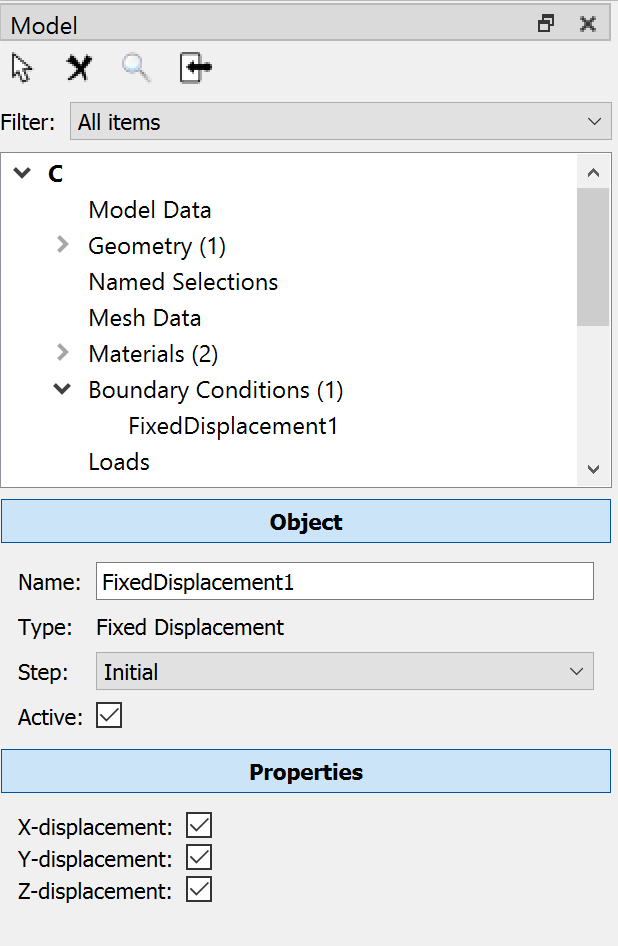
\includegraphics[width=0.22\textwidth]{figuras_2/femur2b.png}
\caption{Fijación de nodos.}
\label{fig:femur2b}
\end{figure}
 
 Al pulsar la tecla \emph{escape} deseleccionamos los nodos seleccionados anteriormente. Procedemos ahora con la condición de contorno de carga. En este caso seleccionamos un nodo en la parte más alta del fémur. El radio de acción escogido en este caso será de 10. La zona seleccionada será similar a la de la figura~\ref{fig:femur3}.
  
  \begin{figure}[!htp]
\centering
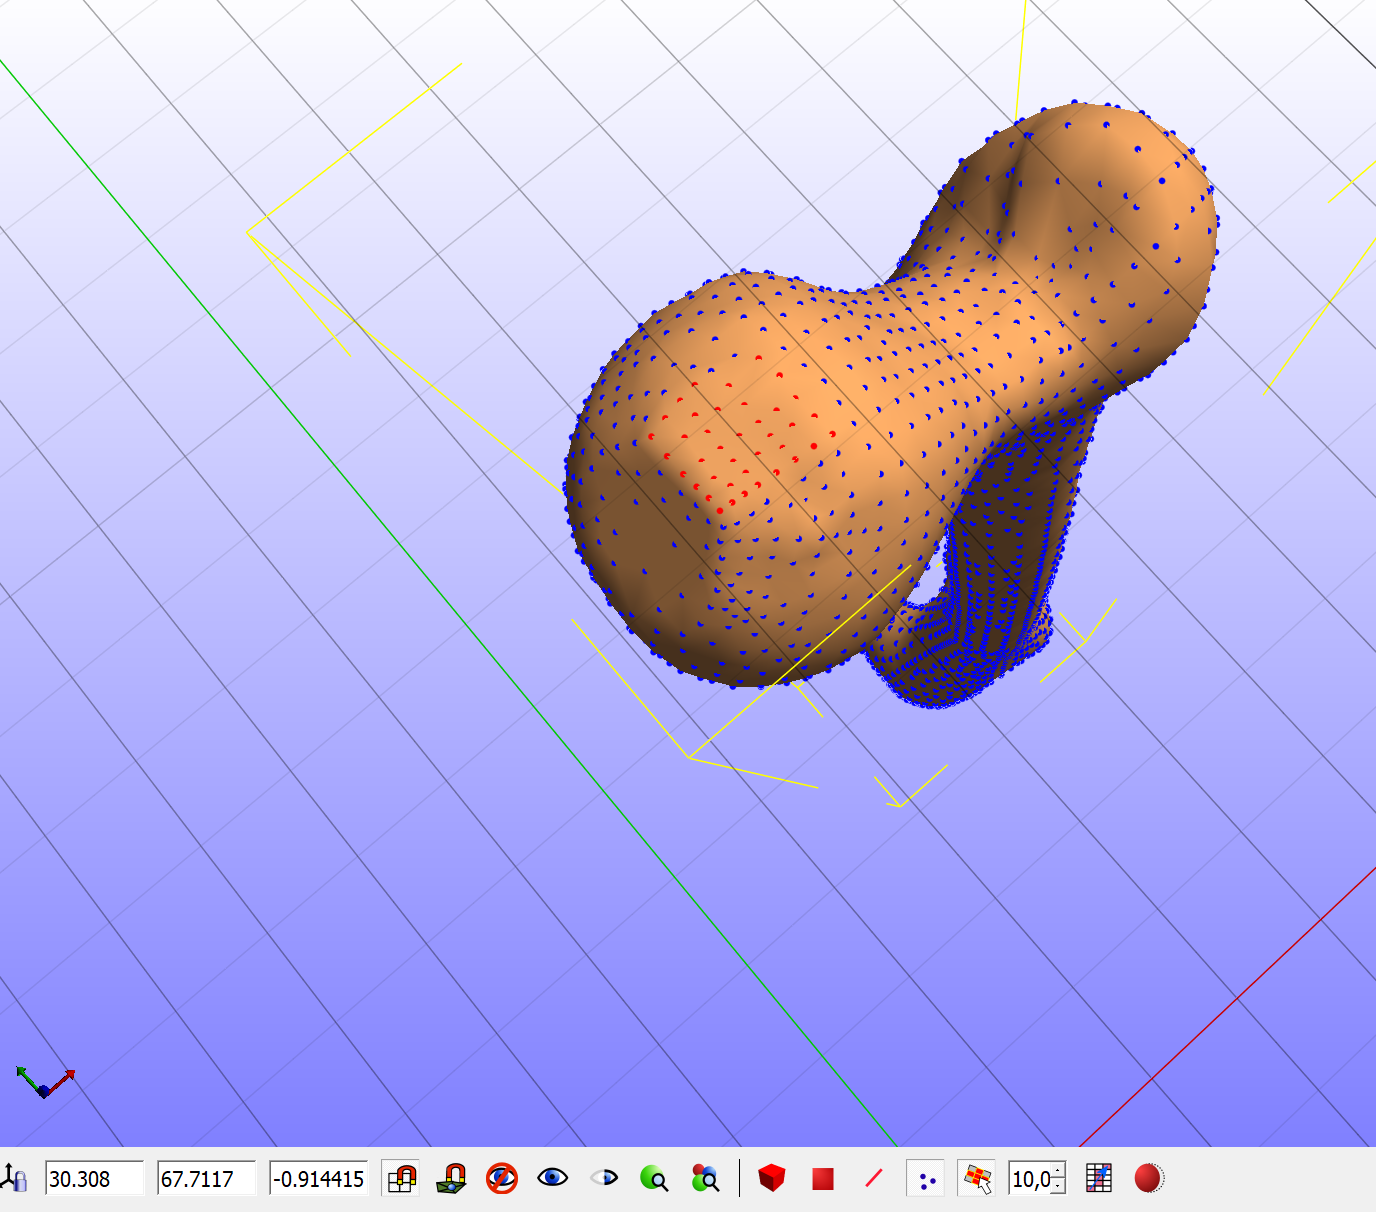
\includegraphics[width=0.85\textwidth]{figuras_2/femur3.png}
\caption{Selección de nodos a cargar.}
\label{fig:femur3}
\end{figure}

Añadiremos una carga nodal desde \emph{Physics/Add Nodal Load}, seleccionando la dirección $z$ y dejando el valor, por ahora, en 1. Se añadirá dicha carga a la sección \emph{Model}. Necesitaremos ahora conocer el número de nodos seleccionados. Cuando lo sepamos hemos de dividir la carga a aplicar, 1000 N entre los nodos a cargar, en el caso del modelo de la figura~\ref{fig:femur3}: 40. Por tanto, cambiaremos el valor de 1 por -25.00, puesto que es el valor del reparto de dicha carga y hemos de darle la dirección negativa en el  eje \emph{z}.

Finalmente, hemos de añadir un \emph{Analysis Step} (\emph{Physics/Add Analysis Step}), que dejaremos el que nos crea por defecto, en 10 pasos de carga. Ahora podremos generar un archivo  de cálculo \texttt{.feb}, con cuidado de cambiar el nombre al que hemos importado para no sobrescribir el mismo. Por defecto lo genera dentro de una carpeta \emph{jobs}, con la siguiente configuración:

\clearpage
 \begin{figure}[!htp]
\centering
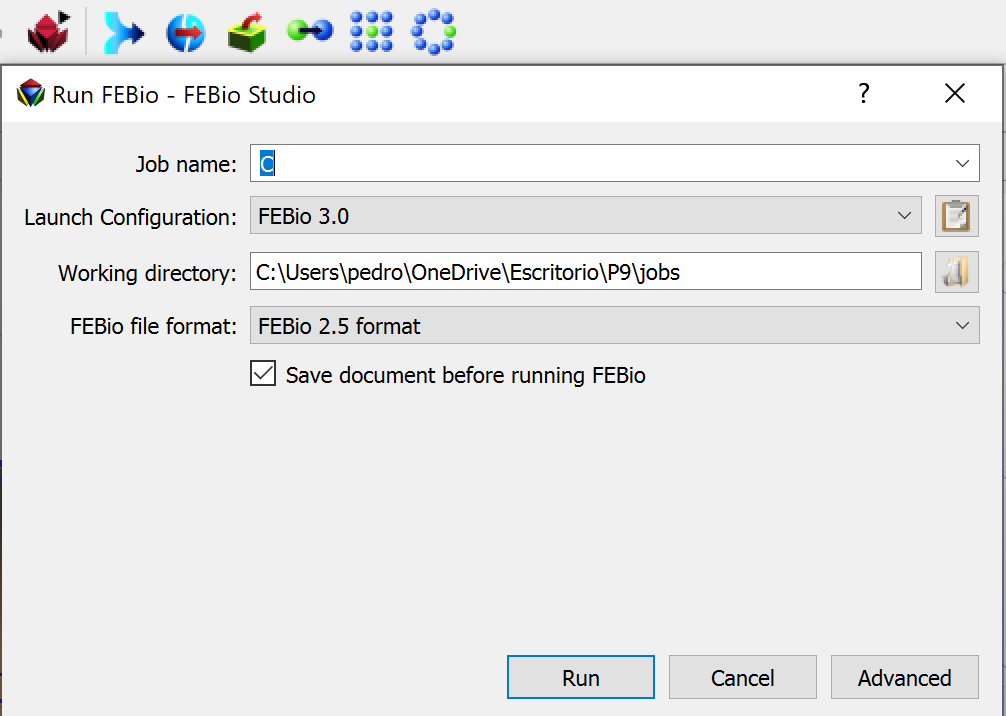
\includegraphics[width=0.5\textwidth]{figuras_2/femur_run.png}
\caption{Creación de archivo de cálculo.}
\label{fig:femur_run}
\end{figure}

Una vez exportado, procedemos a correr la simulación. Cuando esta finalice, podremos abrir el archivo  \texttt{.xplt} generado. Hacemos doble click en el nombre del trabajo creado:

 \begin{figure}[!htp]
\centering
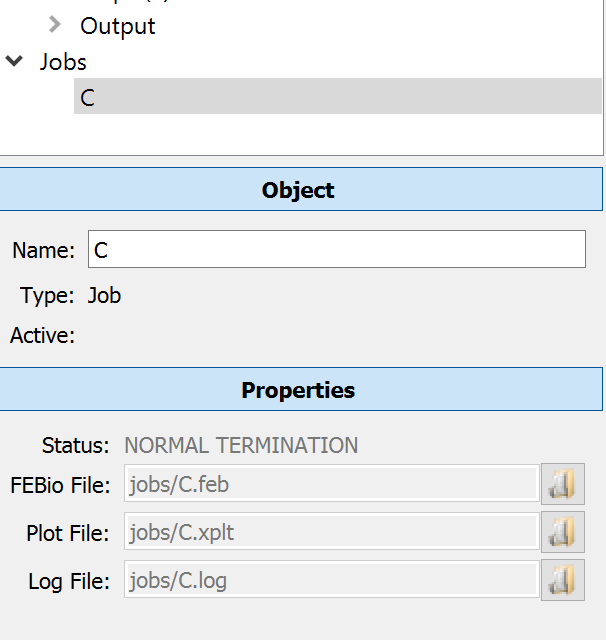
\includegraphics[width=0.3\textwidth]{figuras_2/femur_open.png}
\caption{Paso de Preview a Postview.}
\label{fig:femur_open}
\end{figure}

Una vez abramos el archivo, la ventana cambia a postproceso (\emph{Postview}). Es interesante verificar los materiales de los que se compone nuestro modelo. Para ello, añadimos un corte con la herramienta corte de Postview (señalada en rojo en la figura~\ref{fig:femur4}, y especificamos que el plano sea el normal al eje $y$. Jugando con la distancia al $(0,0,0)$ podemos conseguir una visión similar a la de la  figura~\ref{fig:femur4}.

  \begin{figure}[!htp]
\centering
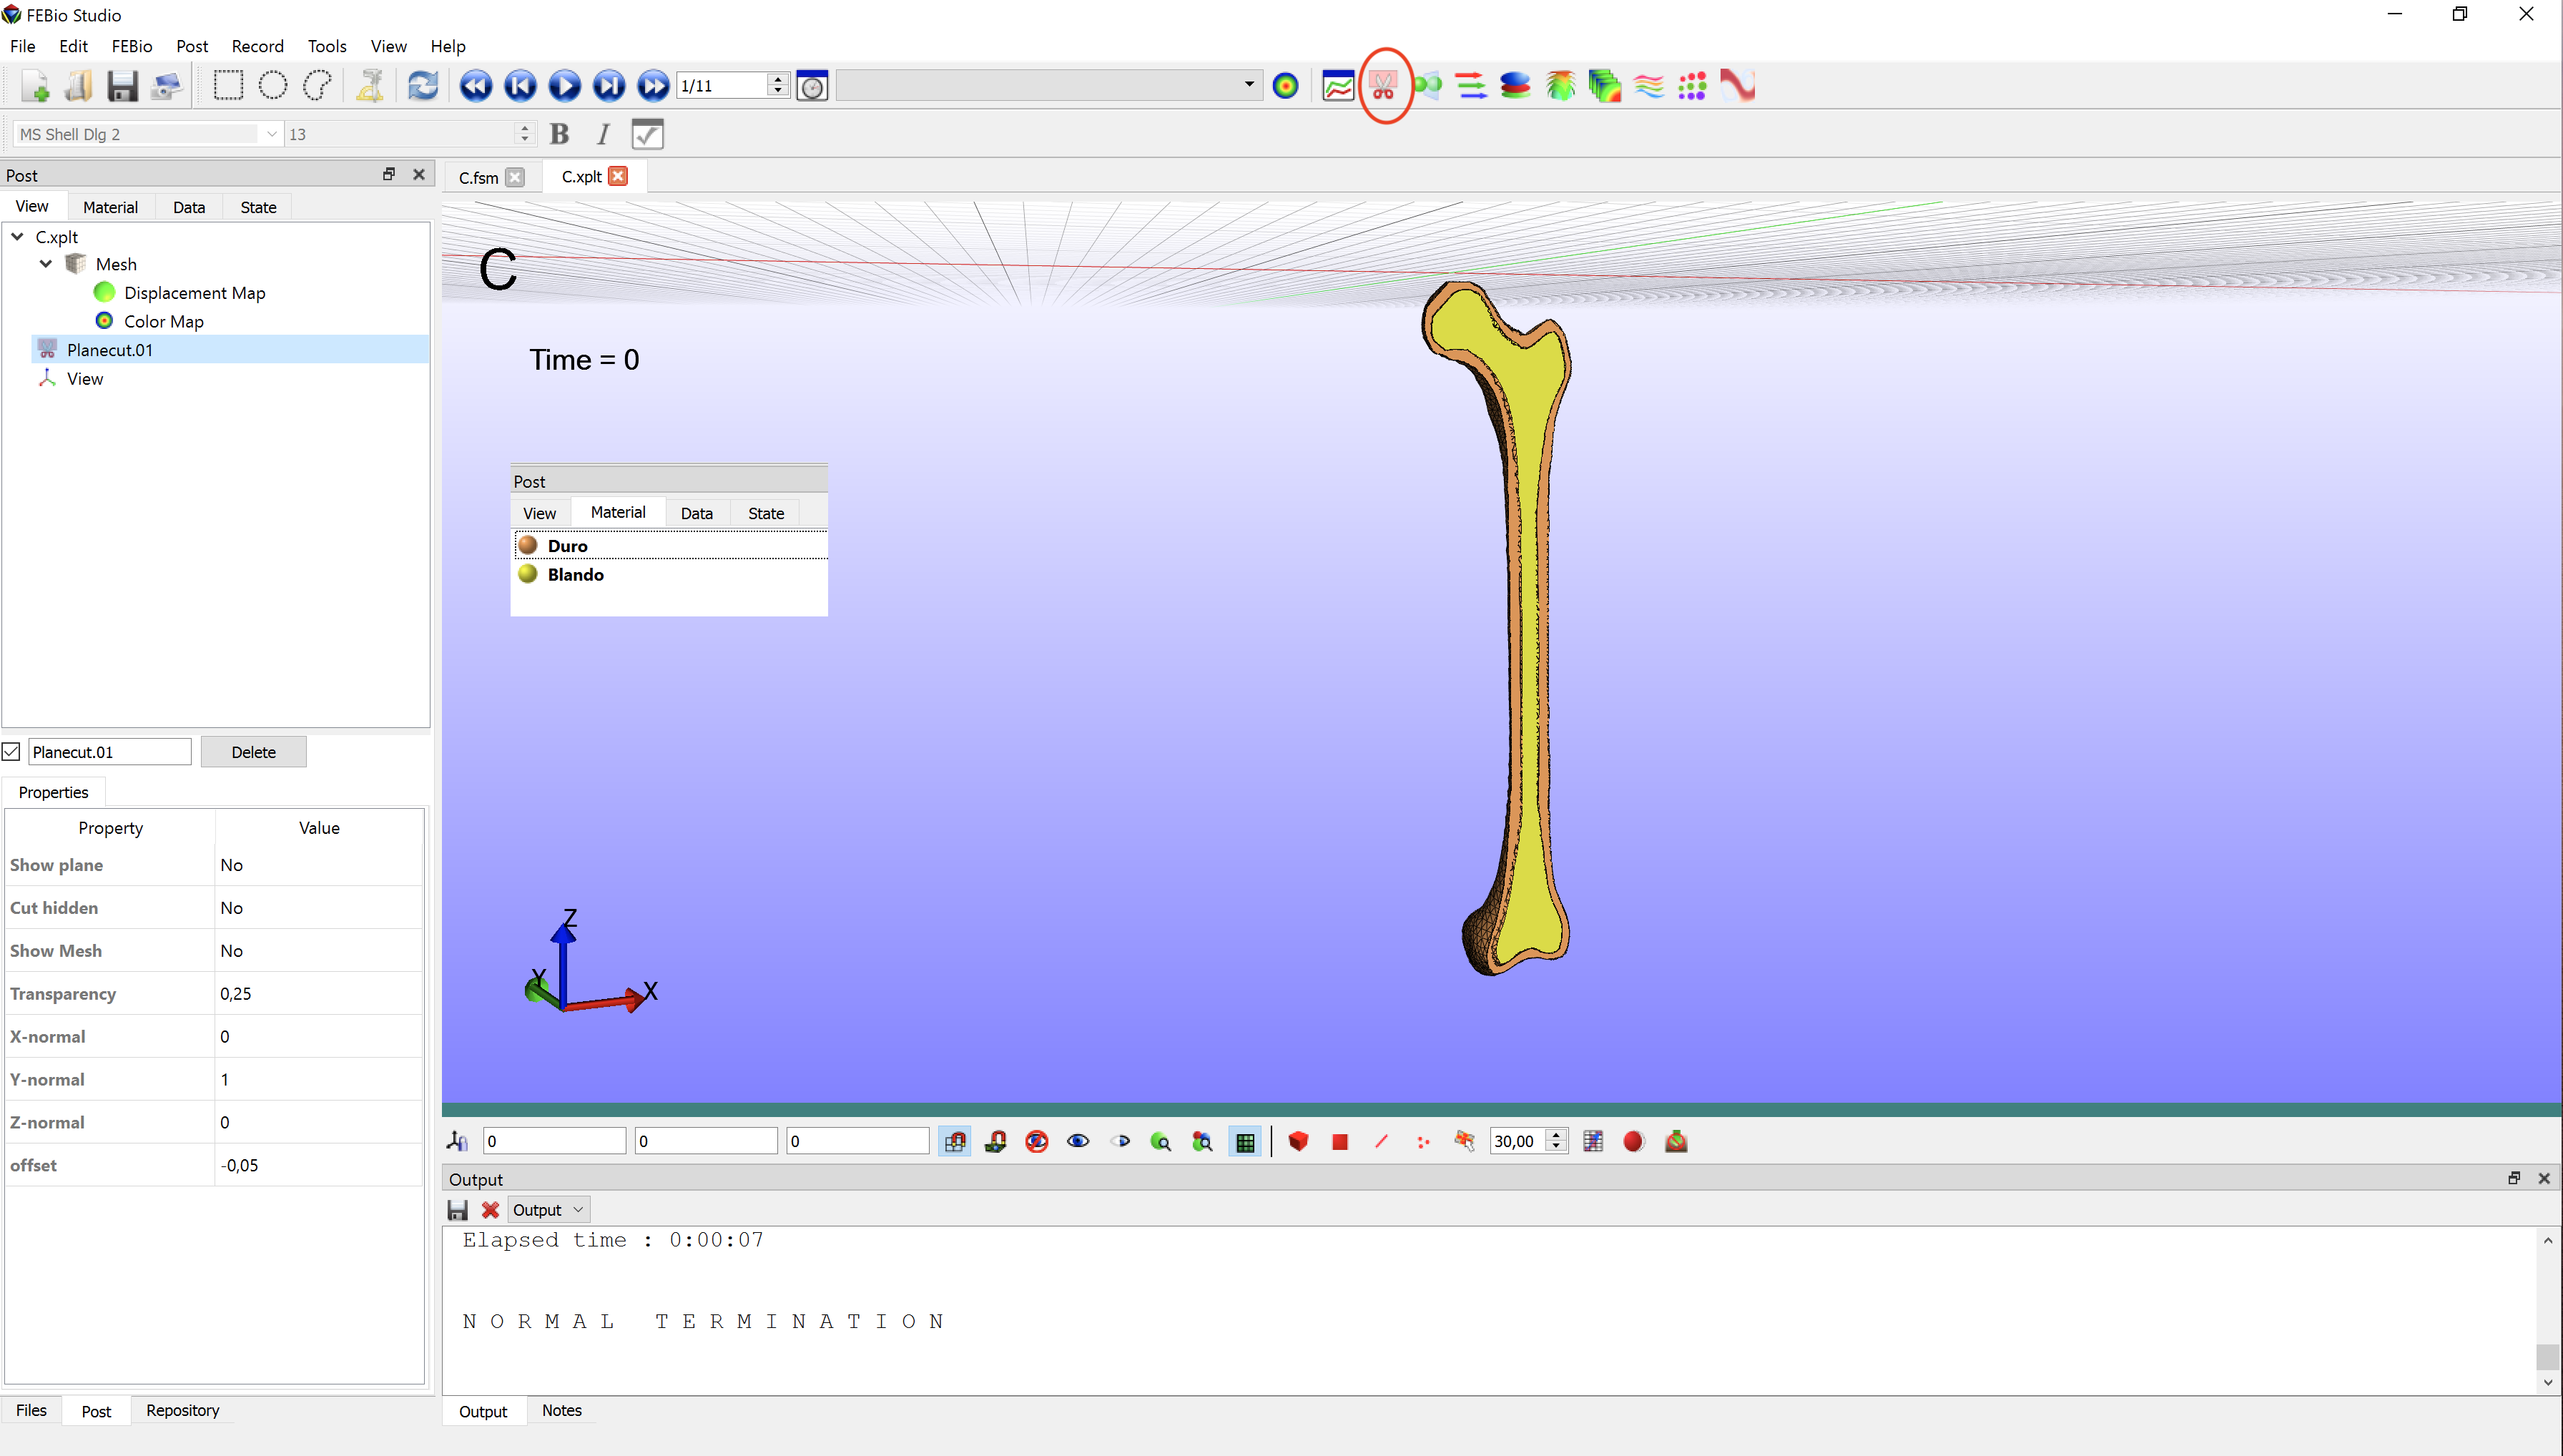
\includegraphics[width=0.95\textwidth]{figuras_2/femur4.png}
\caption{Corte en el plano coronal y esquema de materiales del modelo de fémur empleado.}
\label{fig:femur4}
\end{figure}

A modo de análisis de resultados, en un problema de huesos nos resulta interesante ver en qué puntos puede fallar el tejido oseo. Para ello, nos interesa conocer los valores usuales que usan los criterios de fallo típicos de este material, que serían la tensión efectiva o tensión de von Mises y la tensión principal 1 o tensión principal a tracción. Ambos valores, para el último paso de carga, se pueden observar en la figura~\ref{fig:femur-05-06}.

\begin{figure}[!htp]
\centering
\begin{subfigure}[b]{0.44\textwidth}
\centering
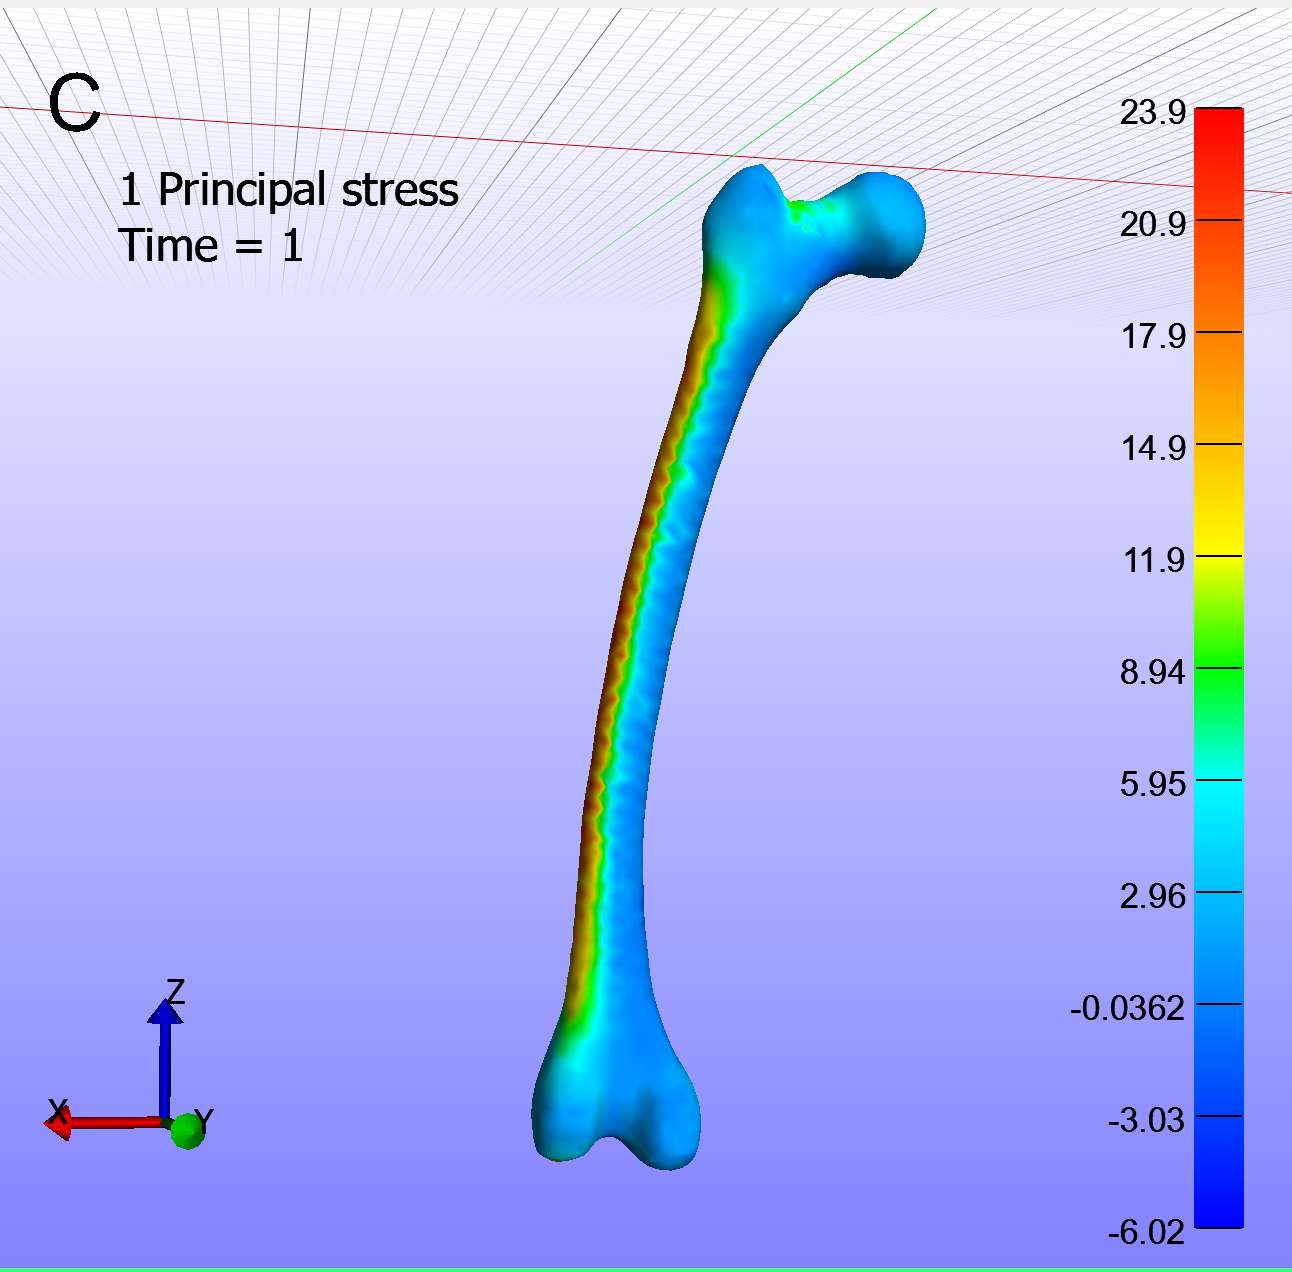
\includegraphics[width=\textwidth]{figuras_2/femur5.png}
\caption{Tensión principal 1}
\label{fig:femur5}
\end{subfigure}
\begin{subfigure}[b]{0.45\textwidth}
\centering
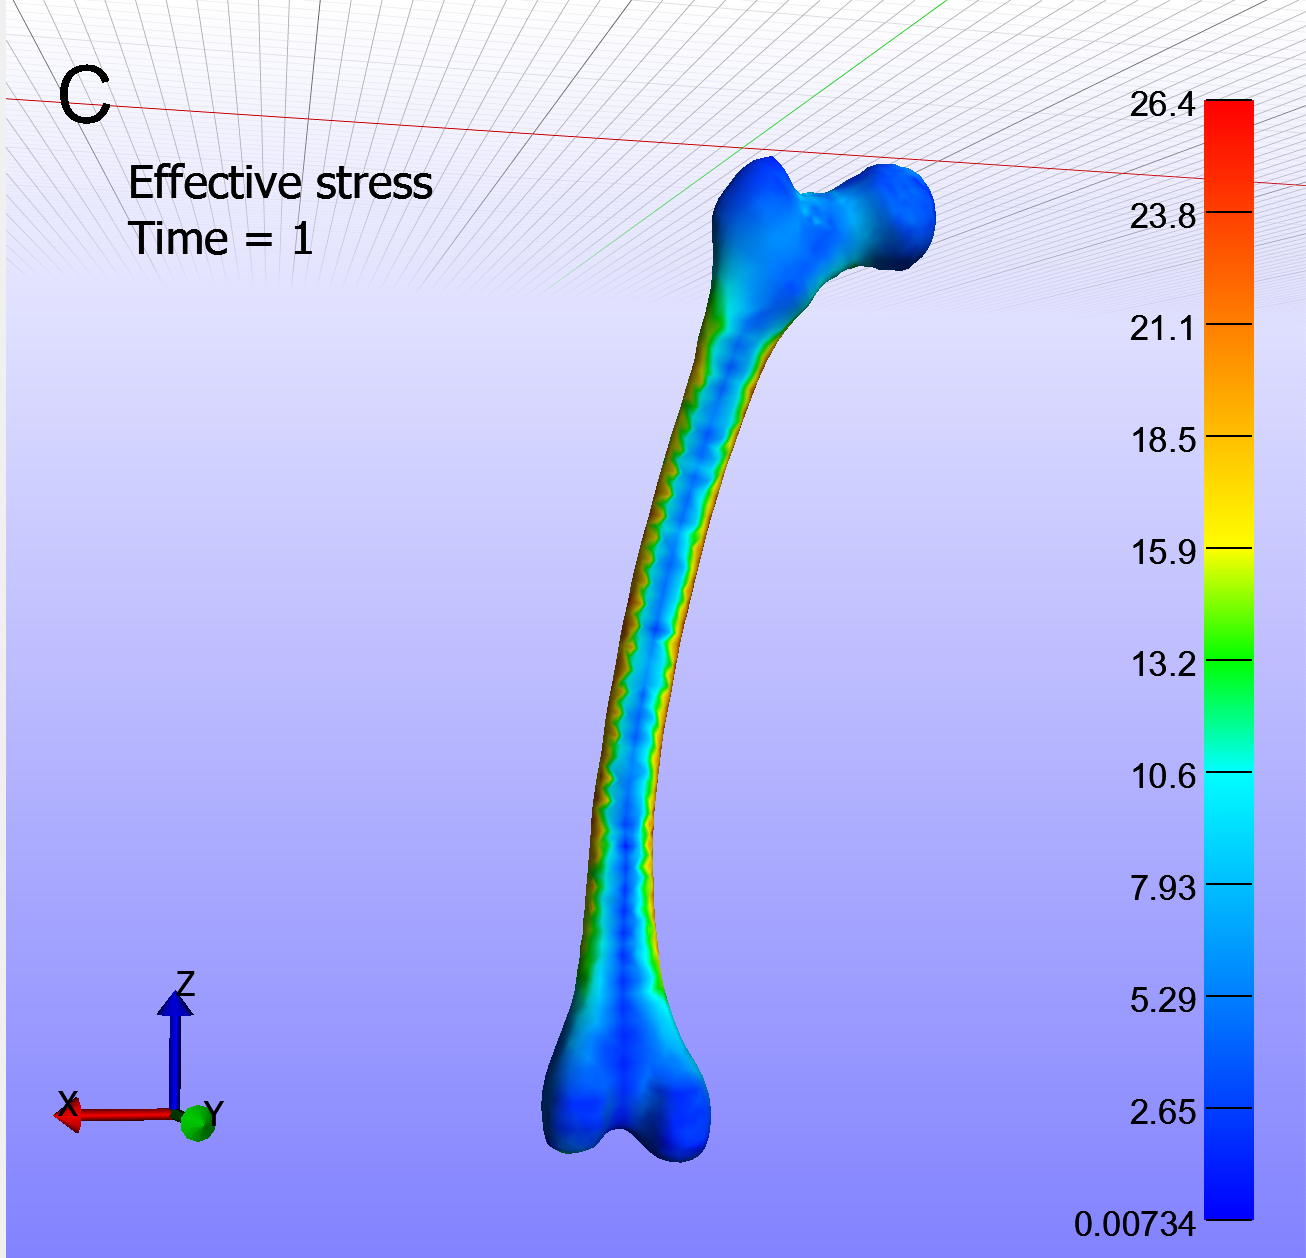
\includegraphics[width=\textwidth]{figuras_2/femur6.png}
\caption{Tensión efectiva}
\label{fig:femur6}
\end{subfigure}
\caption{Resultados de tensiones para el problema real de un fémur sometido a flexión.}
\label{fig:femur-05-06}
\end{figure}


\clearpage
\section{Tareas para entregar}
\label{sec:tareas}

Deberán obtenerse y presentarse los siguientes resultados:
\begin{enumerate}
	\item
	Realizar un estudio de la aplicación de una carga de flexión para la obtención de la carga a la que rompería el tejido oseo. Consideraremos una tensión máxima en compresión de 200 MPa y de 100 MPa en tracción.
	
	\item
	Fichero de video (\texttt{.avi} o \texttt{.mov}) con animación del mapa coloreado de las tensiones más representativas para el caso del fémur.
\end{enumerate}